\chapter{Characterization of the phase plate}
The final goal of this project was to have a complete characterization of the phase plate that we received from the company. We knew its expected behaviour, namely the creation of a top hat potential with the characteristics described in \Cref{sec:slm_phaseplate}. However, it is important to test any new components, to see how they behave in reality.

\section{Building the experimental setup}
\subsection{Imaging system}
In order to characterize the phase plate, the first step was to set up an imaging system. This was necessary to acquire images of the intensity distribution generated by our spatial light modulating system. Since the expected dimensions of the intensity distribution were of the order of \SI{10}{\micro\meter}, a magnification system was set up. The magnification system is composed by a microscope objective, which magnifies the beam, and by a CCD camera. The distance between the two is kept constant by fixing everything in a cage. The objective can be aligned to the beam moving it in the horizontal ($y$) and vertical ($z$) direction by turning two micrometers. A sketch of the setup is shown in \cref{fig:imaging}. The whole system (objective+camera) was mounted on a linear translation stage, with which it could be moved along the $x$ direction to find the focus.

\begin{figure}
    \centering
    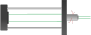
\includegraphics[width=0.65\textwidth]{chapters/chapter_3/figures/imaging}
    \caption{Imaging system. A microscope objective magnifies the image and a CCD camera acquires it. The objective can be moved in the $y$ and $z$ direction with two micrometers.}
    \label{fig:imaging}
\end{figure}

In order to use the imaging system to take measurements, it had to be calibrated. For the calibration, a laser beam was sent to a target like the one shown in \cref{fig:target} and imaged. From the image shown in \cref{fig:magnified}, it was possible to calculate the magnifying power of the imaging system. The lines were measured to be separated by \SI{413(2)}{\micro\meter}. Knowing that on the target the separation was $1/55$~mm, we find a magnifying power of \SI{22.7(1)}{}.

\begin{figure}
    \hfill
    \begin{subfigure}[b]{0.3 \textwidth}
        \includegraphics[width=\textwidth]{chapters/chapter_3/figures/target.jpg}
        \\
        \caption{Target}
        \label{fig:target}
    \end{subfigure}
    \hfill
    \begin{subfigure}[b]{0.55\textwidth}
        \includegraphics[width=\textwidth]{chapters/chapter_3/figures/magnified}
        \caption{Magnified image}
        \label{fig:magnified}
    \end{subfigure}
    \hfill
    \caption{Calibration of the imaging system. On the left, an example of a target similar to the one used in the experiment. On the right, the magnified image of a portion of the target. The number 55 means that the target has 55 lines / \si{mm}.}
\end{figure}

\subsection{Test with the $0-\pi$ phase plate}
\begin{figure}
    \centering
    \includegraphics[width=0.9\textwidth]{chapters/chapter_3/figures/0pi_setup.pdf}
    \caption{Setup for the test of the $0-\pi$ phase plate. The beam coming from the fiber is collimated by a single lens, then expanded by two cylindrical lenses and sent to the phase plate. After the phase plate, an $f=\SI{100}{mm}$ lens is placed and the result is imagined at the focal plane of the last lens. The two cylindrical lenses and the phase plate are mounted on a rotation mount.}
    \label{fig:0pi_setup}
\end{figure}

Before testing the top hat phase plate, the setup was tried with the $0-\pi$ phase plate currently used. In this previous setup, the laser beam coming from a fiber is collimated with a single lens. The beam is then magnified in the $z$ direction by a telescope made of two cylindrical lenses ($f=-40/150$~mm) placed \SI{110}{mm} apart. The magnification of the beam helps to achieve higher trapping frequencies. The beam is then sent to the phase plate and an $f=\SI{100}{mm}$ lens. The two cylindrical lenses and the phase plate are mounted on a rotation mount, to allow the alignment of their axis. The result is imaged by the imaging system at the focal plane of the last lens. The focus is adjusted by moving the imaging system along the $x$ direction with a micrometer. A sketch of this setup is shown in \cref{fig:0pi_setup}.

\begin{figure}
    \centering
    \includegraphics[width=0.5\textwidth]{chapters/chapter_3/figures/0pi_image.pdf}
    \caption{Intensity distribution after the $0-\pi$ phase plate. The size shown on the axis is the real size of the beam. The plots on the right and on top of the image show the integrated sum of the intensity along the respective axes.}
    \label{fig:0pi_image}
\end{figure}


In order to get a good result, it is important that the two cylindrical lenses and the phase plate axes are aligned. To align it, the beam was observed at short and long distances. Acting on the first lens, the beam was rotated in a way such that its axis was aligned vertically. The same alignment was then performed acting on the second cylindrical lens and looking at the beam in the far field. The procedure was repeated, \enquote{walking} the beam, until the two lenses were aligned. The collimation of the beam was ensured by using a shear plate. Finally, the phase plate was aligned rotating its axis in such a way that it was parallel to the beam axis and moving it up or down such that the intensity of the two peaks was the same.

The final result is shown in \cref{fig:0pi_image}. The result resembles the expected $\text{TEM}_{01}$ mode shown in \cref{fig:tem10}, but it is clear that it could be optimized and made more symmetric. In particular, the alignment of the whole setup could have been improved.  However, since the characterization of the $0-\pi$ phase plate was not the goal of the project, the setup was not optimized. Nonethss, this test was useful to gain familiarity on how to work with phase plates, before studying the one we were interested in.



\subsection{Shaping the input beam}
It had already been reported in Schmidt's work that the most crucial parameter to make the phase plate work is the beam diameter \cite{schmidt2021}. The phase plate was ordered for a diameter of \SI{6}{mm}, so this is the first thing we tried to achieve.

\subsubsection{Single collimating lens + x2 telescope}
Initially we tried to collimate the beam coming from the fiber with a single lens with a focal length chosen to produce a \SI{3}{mm} beam. Using a $\times 2$ telescope, composed of a $f=\SI{50}{mm}$ and a $f=\SI{100}{mm}$ achromatic lenses placed \SI{150}{mm} apart, we expected a final beam with a diameter of \SI{6}{mm}. We first tried to collimate the beam with \SI{15.3}{mm} C260-TME-A lens (\cref{fig:beam_f15.3}), but the beam was smaller than \SI{3}{mm}. Then we tried two \SI{18.4}{mm} lens (\cref{fig:beam_f18.4_small,fig:beam_f18.4_large}). The diameter of the former (C280-TMD-A) was too small ($\approx \SI{3}{mm}$), and produced a beam with many aberrations; the latter, with a larger diameter, seemed to solve the problem. The beam was then magnified by the telescope, resulting in the picture shown in \cref{fig:beam_f18.4x2}.

\begin{figure}[t!]
    \begin{subfigure}{0.5\textwidth}
        \includegraphics[width=\textwidth]{chapters/chapter_3/figures/beam_f15.3.pdf}
        \caption{f = \SI{15.3}{mm}}
        \label{fig:beam_f15.3}
    \end{subfigure}
    \begin{subfigure}{0.5\textwidth}
        \centering
        \includegraphics[width=\textwidth]{chapters/chapter_3/figures/beam_f18.4_small.pdf}
        \caption{f = \SI{18.4}{mm}, small diameter}
        \label{fig:beam_f18.4_small}
    \end{subfigure}
    \begin{subfigure}{0.5\textwidth}
        \centering
        \includegraphics[width=\textwidth]{chapters/chapter_3/figures/beam_f18.4_large.pdf}
        \caption{f = \SI{18.4}{mm}, large diameter}
        \label{fig:beam_f18.4_large}
    \end{subfigure}
    \begin{subfigure}{0.5\textwidth}
        \centering
        \includegraphics[width=\textwidth]{chapters/chapter_3/figures/beam_f18.4x2.pdf}
        \caption{f = \SI{18.4}{mm}, x2 telescope}
        \label{fig:beam_f18.4x2}
    \end{subfigure}
    \caption{Beam collimation with a single lens. The focal length of each lens is indicated below the respective figure. In figure (b) and (c) the lenses have the same focal length but different diameter. In figure (d) the beam is magnified with a $\times 2$ telescope.}
\end{figure}

Given the bad result, we decided to try with a different configuration.

\begin{figure}[p]
    \begin{subfigure}{0.5\textwidth}
        \centering
        \includegraphics[width=\textwidth]{chapters/chapter_3/figures/beam_f12.pdf}
        \caption{f = \SI{12}{mm}}
        \label{fig:beam_f12}
    \end{subfigure}
    \begin{subfigure}{0.5\textwidth}
        \centering
        \includegraphics[width=\textwidth]{chapters/chapter_3/figures/beam_f12x3.pdf}
        \caption{f = \SI{12}{mm}, $\times3$ telescope}
        \label{fig:beam_f12x3}
    \end{subfigure}
    \\
    \hfill
    \begin{subfigure}{\textwidth}
        \centering
        \includegraphics[width=0.5\textwidth]{chapters/chapter_3/figures/tophat_f12x3.pdf}
        \caption{Top hat distribution}
        \label{fig:tophat_f12x3}
    \end{subfigure}
    \hfill
    \caption{Beam collimation with a \SI{12}{mm} Schäfter-Kirchhoff collimator, magnified with a $\times3$ telescope ((a) and (b)).  The meaning of the fits in (c) are explained \cref{sec:characterization_methods}.}
    \label{fig:f12mm}
\end{figure}

\subsubsection{Schäfter-Kirchhoff collimator + $\times 3$ telescope}
The second configuration we tried we collimated the beam with a Schäfter-Kirchhoff collimator (60FC-4-M12-10, $f=\SI{12}{mm}$). The collimator was expected to produce a beam with a diameter of $\approx \SI{2}{mm}$, which therefore required a $\times3$ telescope. The telescope was assembled using a \SI{-50}{mm} lens and a \SI{150}{mm} lens. Both lenses were achromatic lenses, to reduce aberrations. The use of a concave and a convex lens, beside reducing aberrations, allowed also to keep the setup more compact. The beams before and after the telescope are shown in \cref{fig:beam_f12,fig:beam_f12x3}.

In \cref{fig:tophat_f12x3} it is also shown the profile of the beam after being shaped by the phase plate in combination with a \SI{100}{mm} lens. It is clear that, despite the general features of the top hat distribution being present, the intensity distribution is very different from the expected one. In particular the top and bottom light sheets seem to be curved around the centre.

\subsubsection{Single collimating lens}
To improve the previous result, we tried to reduce the aberrations using a single achromatic lens to collimate the beam directly to the desired size. In particular, we tried two different lenses: TRH254-040-A-ML ($f=\SI{40}{mm}$) and MG 01LAO785 ($f=\SI{37.5}{mm}$). The results are shown in \cref{fig:beam_single_lens}. Also in this configuration, the beam differs a lot from a clean Gaussian beam.

\begin{figure}[p]
    \begin{subfigure}{0.5\textwidth}
        \centering
        \includegraphics[width=\textwidth]{chapters/chapter_3/figures/beam_f40.pdf}
        \caption{f = \SI{40}{mm}}
        \label{fig:beam_f40}
    \end{subfigure}
    \begin{subfigure}{0.5\textwidth}
        \centering
        \includegraphics[width=\textwidth]{chapters/chapter_3/figures/beam_f37.pdf}
        \caption{f = \SI{37.5}{mm}}
        \label{fig:beam_f37.5}
    \end{subfigure}
    \caption{Beam collimation with a single lens.}
    \label{fig:beam_single_lens}
\end{figure}

\subsubsection{Schäfter-Kirchhoff collimator}
Since we were not able to achieve good results only with the optics we had in the lab, we decided to order a collimator with the desired features. In particular, we ordered a Schäfter-Kirchhoff 60FC-L-4-M35-26 collimator, specifically designed to collimate large beams. In \cref{fig:collimator} we show the beam and the result after it being shaped by the phase plate together with a \SI{100}{mm} lens. Surprisingly, the result is even worse than the previous ones. Placing the phase plate in the far field with respect to the collimator, the result does not change appreciably. Even trying to reduce the aberrations by adding a 1:1 telescope with a pinhole in between, the result remained the same.

\begin{figure}[]
    \begin{subfigure}{0.5\textwidth}
        \centering
        \includegraphics[width=\textwidth]{chapters/chapter_3/figures/beam_f35.pdf}
        \caption{Beam}
        \label{fig:beam_f35}
    \end{subfigure}
    \begin{subfigure}{0.5\textwidth}
        \centering
        \includegraphics[width=\textwidth]{chapters/chapter_3/figures/tophat_f35.pdf}
        \caption{Top hat}
        \label{fig:beam_f37.5}
    \end{subfigure}
    \caption{Beam collimation with a Schäfter-Kirchhoff \SI{35}{mm} collimator. The first image shows the beam after the collimator. The second image shows the top hat distribution generated by the phase plate together with a \SI{100}{mm} lens. The meaning of the fits in (b) are explained \cref{sec:characterization_methods}.}
    \label{fig:collimator}
\end{figure}

\subsubsection{Schäfter-Kirchhoff collimator + $\times 3$ telescope with varying size}

Since even in the (theoretically) best configuration, i.e. using a collimator designed to produce a beam of the desired size, the result was far from optimal, we thought that the problem may have been in the beam size itself. Therefore, we decided to investigate the influence of the beam diameter on the result more systematically. To do so, we went back to the configuration with the chäfter-Kirchhoff \SI{12}{mm} collimator with the $\times3$ telescope, with which we had obtained the best result so far.

To vary the size of beam, instead of using the collimator in its usual way, we manually adjusted it to produce a non-collimated beam. Moving the second lens of the telescope back and forth, it was then possible to re-collimate the beam. In this way, we could vary the size of the beam keeping it collimated at the phase plate  position.

\begin{figure}
    \begin{subfigure}{0.5\textwidth}
        \centering
        \includegraphics[height=0.75\textwidth]{chapters/chapter_3/figures/x3_sizes/beam1.pdf}
        \caption{}
        \label{fig:f12x3_small_beam}
    \end{subfigure}
    \begin{subfigure}{0.5\textwidth}
        \centering
        \includegraphics[height=0.7\textwidth]{chapters/chapter_3/figures/x3_sizes/tophat1.pdf}
        \caption{}
        \label{fig:f12x3_small_tophat}
    \end{subfigure}
    \begin{subfigure}{0.5\textwidth}
        \centering
        \includegraphics[height=0.75\textwidth]{chapters/chapter_3/figures/x3_sizes/beam3.pdf}
        \caption{}
        \label{fig:f12x3_medium_beam}
    \end{subfigure}
    \begin{subfigure}{0.5\textwidth}
        \centering
        \includegraphics[height=0.7\textwidth]{chapters/chapter_3/figures/x3_sizes/tophat3.pdf}
        \caption{}
        \label{fig:f12x3_medium_tophat}
    \end{subfigure}
    \begin{subfigure}{0.5\textwidth}
        \centering
        \includegraphics[height=0.75\textwidth]{chapters/chapter_3/figures/x3_sizes/beam2.pdf}
        \caption{}
        \label{fig:f12x3_large_beam}
    \end{subfigure}
    \begin{subfigure}{0.5\textwidth}
        \centering
        \includegraphics[height=0.7\textwidth]{chapters/chapter_3/figures/x3_sizes/tophat2.pdf}
        \caption{}
        \label{fig:f12x3_large_tophat}
    \end{subfigure}
    \caption{Beam and top hat distribution for different beam sizes. Every row shows a beam on the left and its respective top hat distribution on the right. The results were obtained
        with the \SI{12}{mm} collimator and together with the $\times3$ telescope. The meaning of the fits on the top hat images are explained \cref{sec:characterization_methods}.}
    \label{fig:f12x3_sizes}
\end{figure}

The results, for three different sizes of the beam, are collected in \cref{fig:f12x3_sizes}. From the figures, it is clear that the dimension of the beam has a big influence on the result. Even changes of fractions of a millimetre produce great differences in the final result. In particular, it is interesting to observe that for large beams we recognize the behaviour observed in all the previous configurations, i.e. a curvature of the two peaks around the centre. On the other hand, small beams produce an uneven intensity distribution along the $y$ axis, with peaks at the border of the flat region. A good compromise seems to be found for a beam of $\approx \SI{5}{mm}$. This explains the bad results obtained before, since we were using much larger beams, even if the size was similar to the specifications given by the manufacturing company.

Having found a good beam size which we could aim for, we decided to build a telescope that would give us approximately the desired size, and use it to fully characterize the phase plate.

\section{Characterization}
\label{sec:characterization}
For the characterization of the phase plate we decided to keep using the Schäfter-Kirchhoff \SI{12}{mm} collimator, but instead of magnifying the beam with a $\times3$ telescope, we used a $\times2.5$ telescope. With this setup, we expected a beam with a diameter of $\approx \SI{5}{mm}$, size for which we had previously found the best results. The telescope was built with a \SI{-50}{mm} and a \SI{120}{mm} achromatic lenses.

\subsection{Methods}
\label{sec:characterization_methods}
For a complete characterization of the phase plate, it was necessary to analyse its behaviour for different beam sizes and different distances from the focus. It is important to look at the light sheet at different distances from the focus because, despite the focal point being in principle well-defined, it is non-trivial to find it. Moreover, it may happen that for our goals a non-perfectly focused beam is better than a focused one.

\subsubsection{Intensity normalization}

For every combination of beam size and distance from the focus, two pictures were taken: a normal (non-satuaretd) picture and a saturated picture. The non-satuaretd picture gives us information on the intensity distribution for the whole light sheet. The saturated picture allows us to increase the dynamic range in the dark region at the centre, allowing more precise measurements. An example of a saturated picture can be found in \cref{fig:parabola_imsat}. To saturate the picture we increased the exposure time. Taking note of both the exposure time of the saturated picture and of the non-satuaretd one, it was possible to \enquote{normalize} the saturated picture as
\begin{equation}
    I_\text{s}^\text{norm} = \frac{\tau_\text{ns}}{\tau_\text{s}} I_\text{s}
\end{equation}
where $\tau_\text{ns/s}$ are respectively the exposure time of the non-saturated and saturated pictures, $I_\text{s}$ the intensity measured by the camera for the saturated picture and $I_\text{s}^\text{norm}$ the normalized intensity.

For both pictures, the absolute intensity $I_\text{abs}$ was found scaling the intensity measured by the camera $I_\text{rel}$ (already normalized for the saturated image) with a factor given by the power of the laser $P$ divided by the total power measured by the camera
\begin{equation}
    I_\text{abs}(y,z) = P\frac{I_\text{rel}(y,z)}{
        \int \differential y' \differential z' I_\text{rel}(y',z')}
\end{equation}
For all the following calculations, we assumed to have a laser with a power of $\SI{1}{W}$.

\subsubsection{Global behaviour}
The expected intensity distribution generated by the phase plate $I(y,z) = I_\text{th}(y) I_{0\pi}(z)$ is given by a top hat distribution $I_\text{th}(y)$ in the $y$ direction and by a $0-\pi$ distribution $I_{0\pi}(z)$in the $z$ direction. The top hat distribution is given by

\begin{equation}
    I_\text{th}(y) =
    \begin{cases}
        \exp\left[-\left(\frac{\left|y\right|-w_F}{w_R}\right)^2\right] & \quad |y| > w_F    \\
        1                                                               & \quad |y| \leq w_F
    \end{cases}
\end{equation}
where we have defined $2w_F$ as the length of the flat region and $w_R$ the length of the ramp-up. The $o-\pi$ distribution is given by
\begin{equation}
    I_{0\pi}(z) =  \erfi\left[\frac{z}{w_e}\right]^2 \exp\left[-2 \left(\frac{z}{w_e}\right)^2\right]
\end{equation}
where $\erfi(z) = -i\erf(iz)$ is the imaginary error function and $w_e$ an appropriate length scale. It is possible to notice that the $\erfi$ distribution has two peaks distanced by $2w$.

Since the two variable $(y,z)$ of the intensity distribution $I(y,z)$ are theoretically independent, we can gain some first information looking at the integrated sum of the intensity along the two axis
\begin{align}
    I_z(y) & = \int \differential z' I(y,z') \\
    I_y(z) & = \int \differential y' I(y',z)
\end{align}
fitting the respective distributions $I_\text{th}(y)$ and $I_{0\pi}(z)$. This is what was done, for example, in \cref{fig:f12x3_medium_tophat}, where we found a flat region length $2w_F$ of \SI{42.1}{\micro m} and an $\erfi$ distribution with the two peaks distanced by $2w_e = \SI{19.1}{\micro m}$.

The integrated intensity $I_z(y)$ can also be used to calculate a first quantity useful to quantify the \enquote{flatness} of the top hat, the so-called peak-to-peak (P2P). The P2P is simply defined as the minimum intensity in the flat region divided by the maximum
\begin{equation}
    \text{P2P} = \min_y(I_z(y)) / \max_y(I_z(y)) \qquad |y| < w_F
\end{equation}
The closer the P2P is to one, the flatter the top hat distribution is.

\subsubsection{Local behaviour}
Even if the previous analysis give us a good understanding of the global characteristic of the intensity distribution, it fails to be precise about the exact behaviour at the point we are mostly interested in: the central region. Since the atoms will be trapped in this region, ideally in a 2D space, they will only feel the local potential near $z=0$. It is therefore important to characterize this region with more precision.

We have already mentioned in \cref{sec:slm_specifications} that two important quantities for the characterization of the phase plate are the darkness $D$, defined in \cref{eq:darkness}, and the trapping frequency $\omega_z$, defined in \cref{eq:trapping_frequency}. If these two quantities are evaluated for every $y$, their mean and their variation will give us information on the darkness of the region, on the strength of the trapping potential and on the uniformity of the intensity.

To compute these quantities, using the saturated picture, we fit a parabola for every $y$. We can then use the quadratic coefficient to compute the trapping frequency and the height of the vertex to compute the darkness. An example is shown in \cref{fig:parabola}.

\begin{figure}
    \begin{subfigure}{0.45\textwidth}
        \centering
        \includegraphics[height=5.25cm]{chapters/chapter_3/figures/fitquad_imsat.pdf}
        \caption{Saturated image}
        \label{fig:parabola_imsat}
    \end{subfigure}
    \begin{subfigure}{0.55\textwidth}
        \includegraphics[height=5.25cm]{chapters/chapter_3/figures/fitquad.pdf}
        \caption{Quadratic fit}
        \label{fig:parabola_fit}
    \end{subfigure}
    \caption{Example of the quadratic fit of a slice of a saturated image. The slice is taken at $y=\SI{-4}{\micro m}$.}
    \label{fig:parabola}
\end{figure}